\section{Ergebnisse und Ausblick}

\begin{frame}{Forschungsfragen}
  \begin{description}[4cm]
    \item[F1] Welche Konsistenzbeziehungen bestehen zwischen BPMN- und BROS-Modellen?
    \begin{itemize}
      \item Fünf Konsistenzregeln aufgestellt
    \end{itemize}

    \item[F2] Wie lassen sich die Konsistenzbedingungen automatisiert überprüfen?
    \begin{itemize}
      \item Tool als Referenzimplementierung erstellt
    \end{itemize}

    \item[F3] Mit welchem Aufwand ist dieses Verfahren erweiterbar?
    \begin{itemize}
      \item Regelerweiterbarkeit: leicht
      \item Modellerweiterbarkeit: aufwändig
    \end{itemize}
  \end{description}
\end{frame}

\begin{frame}{Klassifikationsschema}
  \begin{table}
  \centering
  \begin{adjustbox}{width=.6\linewidth,center}
    \begin{threeparttable}
      \centering
      \begin{tabular}{p{1.58cm} p{1.50cm} p{0.95cm} p{2.2cm} p{1.60cm} p{0.33cm}
          p{0.33cm} p{0.33cm} p{0.8cm} p{0.8cm}}
        &
        \rot{Diagrams} &
        \rot{Consistency} \rot{Type} &
        \rot{Consistency} \rot{Strategy} & 
        \rot{Intermediate} \rot{Representation} & 
        \rot{Case Study} & 
        \rot{Automatable} & 
        \rot{Tool Support} & 
        \rot{Model} \rot{Extensibility} & 
        \rot{Rule} \rot{Extensibility} \\
        \toprule
        Rasch 2003    & CD, SM              & Intra            & Monitoring           & CSP/OZ                      & \f{1}      & \f{H}       & \f{0}        & \f{H}               & \f{M}              \\
        \midrule
        Shinkawa 2006 & UCD, CD, SD, AD, SC & Inter            & Analysis             & CPN                         & \f{0}      & \f{H}       & \f{0}        & \f{M}               & \f{L}              \\
        \midrule
        Mens 2005     & CD, SD, SC          & All              & Monitoring           & Extended UML                & \f{1}      & \f{H}       & \f{1}        & \f{H}               & \f{M}              \\
        \midrule
        Egyed 2001    & CD, OD, SD          & Intra, Inter     & Construction         &                             & \f{0}      & \f{H}       & $\sim$       & \f{M}               & \f{M}              \\
        \midrule
        Egyed 2006    & CD, SD, SC          & Intra            & Monitoring           &                             & \f{1}      & \f{H}       & \f{1}        & \f{L}               & \f{M}              \\
        \midrule
        BROS          & BPMN, BROS          & Intra            & Monitoring           &                             & \f{1}      & \f{H}       & \f{1}        & \f{L}               & \f{H}  
      \end{tabular}
      \begin{tablenotes}
        \item \hfil
        \f{H}: mit geringem Aufwand;
        \f{M}: mit mittlerem Aufwand;
        \f{L}: mit hohem Aufwand;
        \item \hfil
        \f{1}: ja;
        \f{0}: nein;
        $\sim$: teilweise;
        \item \hfil
        CD: Class Diagram;
        SM: State Machine;
        USC: Use Case Diagram;
        \item \hfil
        SD: Sequence Diagram;
        AD: Activity Diagram;
        SC: Statechart
      \end{tablenotes}    
    \end{threeparttable}
  \end{adjustbox}
  \label{tab:Klassifikationsschema}
\end{table}
\end{frame}

\section{Demo}

\begin{frame}{Demo - Übersicht der Änderungen}
  \begin{figure}
    \centering
    \begin{adjustbox}{width=0.9\linewidth,center}
      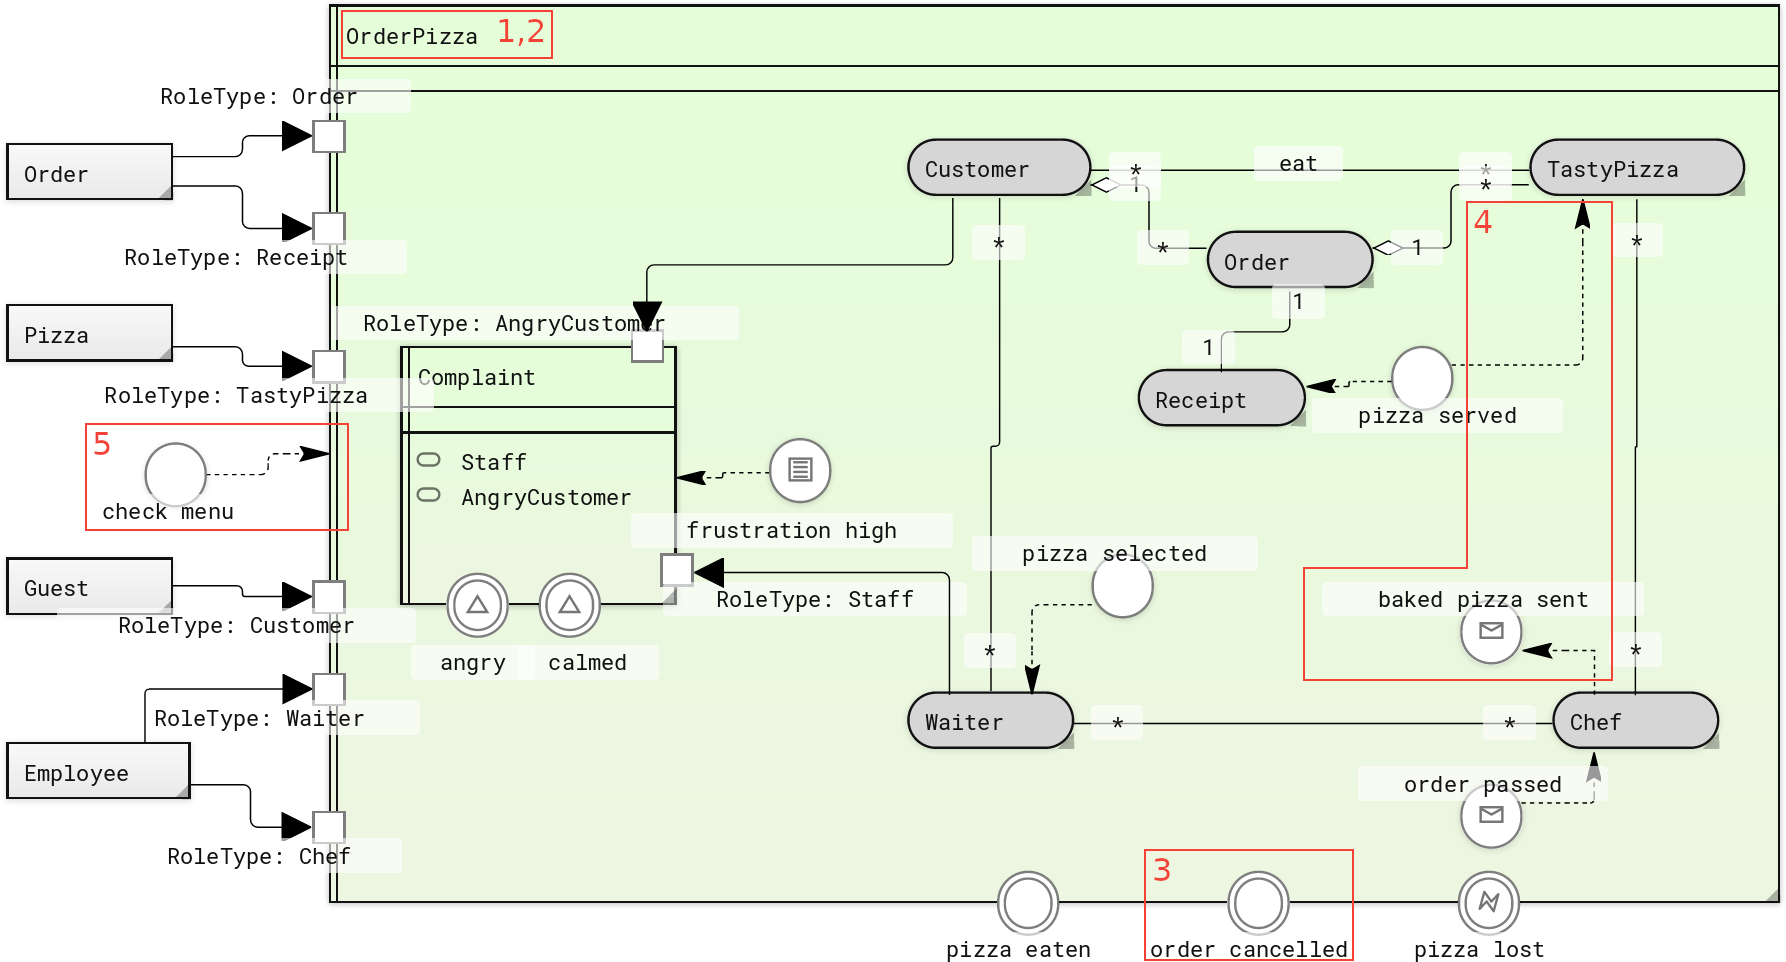
\includegraphics{images/example/bros-rule6H.png}
    \end{adjustbox}
  \end{figure}
\end{frame}

\begin{frame}[allowframebreaks]{Quellen}
  \setquotestyle{english}
  \printbibliography[heading=none]
\end{frame}

\begin{frame}[standout]
  Fragen?
\end{frame}
